\section{The underlying meaning.}

Our explanation so far has relied on analythic methods, and, although consistent within itself, one could reasonably argue that it is as obscure as any other one. We now give each concept semantical meaning, such that the reader comes out convinced that what has been seen until now is not only fair, but also somewhat intuitive.

\subsection{Exponential phenomena.}

One of the ways we can categorize different magnitudes is by how they change and develop. The age of a person increases linearly, this means that it doesn't matter whether someone turns 19 or 91, neither whether that happens in 2025 or in 1320; in every case, the rate of change has remained constant: one year per year.

We say a variable grows \textit{exponentially} when its rate of change is proportional to the value of the variable itself. That is, if the variable is equal to 3, then its rate of change will be proportional to 3. This doesn't seem very impressive until you stop to consider its implications and run the numbers. An example of exponential growth (also called \textit{geometric growth} when talking about discrete cases) is the sequence:

$$1, 4, 16, 64, 256, 1024, 4096, 16384...$$

Note that already on the fith term we're on four figures.

We've previously said that real exponents make no sense (at least before introducing the $\exp(x)$ and $\ln(x)$ functions). While this holds true, it is also true that many real world continuous phenomena exhibit an exponential nature. If we stand faithful to our scientific spirit of inquiry, these kind of phenomena should be taken into account before any notion of $\ln(x)$ and $\exp(x)$ is developed. Let us just create a fiction in which, in some way, we got to a formalisation of real exponents that doesn't have anything to do with these two functions, for example, by \enquote{filling in the holes} in the function $f(x) = 4^x$ for $x \in \mathbb{Q}$ such that $x\in \mathbb{R}$ (making it continuous).

We can analyse the derivative of $f(x) = 4^x$ to find its rate of change and get that:

$$f'(x) = 4^x \cdot 1.386294...$$

As expected, its rate of change is proportional to its value, however, the proportionality constant ($1.386294...$) is quite bizarre. It's also worth saying that this proportionality constant varies depending on the base of the exponential. If we had instead used $g(x) = 7^x$, we would've found that

$$g'(x) = 7^x \cdot 1.945910...$$

\newpage

A natural question that comes to mind when pondering about how one would express this constant in terms of the base is to find a base which makes the constant equal to $1$, this means, not only having an exponential function whose rate of change is \textit{proportional} to its current value, but also one that makes it \textit{exactly equal} to its current value. Surprisingly, the value of this base turns out to be $h(x) = e^x$.

$$h'(x) = e^x$$

Knowing this, we can derive the general expression for the derivative of $F(x) = a^x$. First, note that

$$e^{\log_e(a)} = a$$

This has NOTHING to do with the $\ln(x)$ function. Think of $\log_e(a)$ as any other logarithm which just happens to have base $e$. You can formulate it in the usual \enquote{To what power do you have to raise the number $e$ to get $a$?}. We are allowed to write then that

$$F(x) = a^x = [e^{\log_e(a)}]^x = e^{\log_e(a)\cdot x}$$

If we take its derivative and apply the chain rule,

$$F'(x) = e^{\log_e(a)\cdot x} \cdot \log_e(a)$$

(We know $e^x$ to be its own derivative because that's pretty much how we've defined $e$). Substituting back $a^x$, we get that

$$F'(x) = (a^x)' = a^x \cdot \log_e(a)$$

Recovering the knowledge we obtained from previous sections, it is possible to rewrite this as

$$(a^x)' = a^x \cdot \ln(a)$$

But notice that this is somewhat retconning. The function $\log_e(x)$ isn't the same as $\ln(x)$, as the former works on the realm of rational numbers, whereas the latter works with real numbers. Only after having defined what $\ln(x)$ is can we extend $\log_e(x)$ to mean $\ln(x)$.

Rest assured, after having rigorously defined and proved everything, we can write things in whatever order we want, but this must only be done once the student has a solid understanding on why these backwards compatibilities work.

On a less technical note we would like to point out that choosing $e^x$ to represent exponential phenomena in disciplines like physics or statistics is a merely aesthetical choice. One could very much express $2^3$ as $\pi^{\log_{\pi}(2)\cdot 3}$, it's just that when choosing $e^x$, only the non-cluttering constants --- the ones with actual semantic meaning in the universe --- remain.

\newpage

Take exponential decay. If you have a radioactive material, you can measure how many radioactive isotopes it has ($N_0$). With the passage of time ($t$), some of those isotopes will undergo radioactive decay, transforming into other elements or isotopes and leaving a smaller amount of radioactive isotopes in the material ($N(t)$). This process is also an exponential, and thus can be expressed by the following differential equation:

$$N'(t) = -\lambda N(t)$$

One possible solution to this equation is

$$N(t) = N_0 a^{-ct}$$

Where $c = \lambda \cdot \log_a(e)$. This is, by all means, a valid solution. It's only problem, as we've said, is an aesthetic one. What does $c$ mean? Would one know anything about the phenomenon being described just by glancing at this constant? Absolutely not. If we instead express it this way

$$N(t) = N_0 e^{-\lambda t}$$

Suddenly there are no \enquote{clutter constants} and, more importantly, $\lambda$ takes semantic meaning. In the case of radioactive decay, $\lambda$ is called the \textit{disintegration constant} or \textit{rate constant}. This is not only meaningful for $\lambda$ itself, but for all the magnitudes derived from $\lambda$. For example, $t_{1/2} = \frac{\ln(2)}{\lambda}$ is called the \textit{half life} of the quantity, and it describes the amount of time necessary for the amount $N$ to be cut in half. Could have we expressed the same thing by carrying a factor of $log_a(e)$ the whole time? Absolutely, but then our definition of half life would be something like \enquote{the amount of time necessary for the amount $N$ to be cut in half divided by $\log_a(e)$}. This definition just feels wrong and muddled, whereas the other one seems to carry some objective meaning, as if the constant $e$ was just the \textit{natural} option for deciding a base. This is what makes the natural logarithm \textit{natural}.

To summarize, exponential variables are those whose rate of change is proportional to the variable's value itself, and $e$ is the number which satisfies that that proportionality constant is $1$, which makes it the \textit{natural} way of expressing many equations in physics.

\subsection{Complex numbers as rotations.}

When first introduced to complex numbers, one of the first strange decisions that stand out about their definition is their position on the complex plane. Although any ordered pair can be plotted in a graph, it doesn't seem obvious why $i$ should be one step up from $0$ perpendicular to the real axis. However, when we shift our perspective on numbers to thinking of them as \textit{actions}, this not only becomes a reasonable outcome, but the only possible one.

If one is familiar with simple $\mathbb{R}^2$ vectors, one will already see how numbers can be seen this way. Multiplying a vector by a positive number is \textit{scaling} it, making it bigger or smaller while preserving the way it \enquote{points} to. Similarly, multiplying it by a negative number is doing the same thing but also \enquote{flipping} its direction, or rotating it by $180^{\circ}$.

But what is a $180^{\circ}$ rotation if not two consecutive $90^{\circ}$ rotations? If multiplying by $-1$ yields a $180^{\circ}$ rotation, whatever number represents a $90^{\circ}$ rotation must be, in a sense, the square root of $-1$. This notion of multiplication (of numbers) turning into addition (of angles) should already give away a hint that exponentials will sooner or later be useful as a model.

If one isn't convinced by this argument, note the following. If $z = a + bi$, then $i\cdot z = -b + ai$. This coordinate transformation is exactly the same as a $90^{\circ}$ counter-clockwise rotation ($(x, y) \to (-y, x)$). This concept can be expanded further onto other complex numbers, however our case only requires for us to understand the action of $i$.

\subsection{Complex exponentials.}

This is perhaps the hardest part of all to visualize, so we shall use a physics analogy. It can be useful to interpret $f(t) = \exp(it)$ as the position of a particle in the complex plane at a given point in time, and its derivative $f'(t) = i\exp(it)$ as its velocity. It is worth noting that, at every position, the particle's velocity vector forms a $90^{\circ}$ angle with its position vector (because $f'(t) = i\cdot f(t)$, that is, a $90^{\circ}$ counter-clockwise rotation). One can visualize the particle \enquote{orbiting} the origin in a circular motion (Figure \ref{rot}).

\begin{figure}[H]
	\centering
	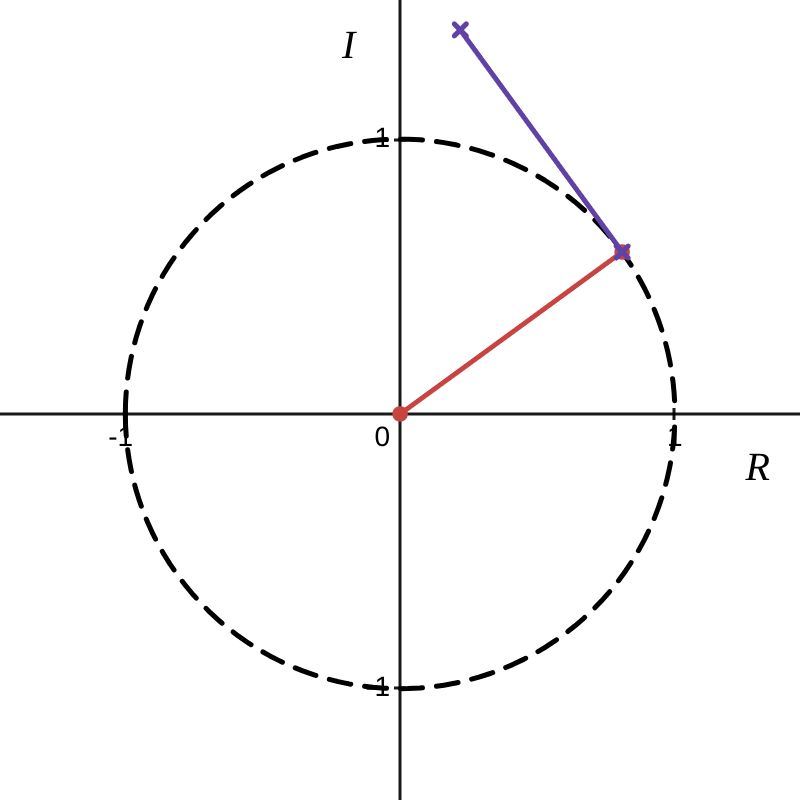
\includegraphics[width=\linewidth]{media/rotation.png}
	\caption{Particle on the complex plane with position $\exp(it)$ (shown in red) and velocity $i\exp(it)$ (shown in purple). In the beginning, $f(0) = 1$. After an infinitesimal nudge in time, the particle will move perpendicular to its position vector (along its velocity vector). As we know from physics, this is the setup for circular motion. An interactive Desmos graph is available at \url{https://www.desmos.com/calculator/8npnlxgjba}.}
	\label{rot}
\end{figure}

What Euler's formula tells us is that the angle the particle's position vector has swept at time $t$ is \textit{exactly} $t$. So, after 2 seconds, the particle forms a 2 radian angle with the real axis; after $\pi$ seconds, the particle forms a $\pi$ radian angle with the real axis (which coincides with the point $-1 + 0i$), etc.

Once again, the exponential function here is not a fundamental choice. We could've chosen the golden ratio $\phi$ as a base, making $f(t) = \phi^{it}$ and $f'(t) = \ln(\phi) \cdot \phi^{it}$. The only difference is that in this case the swept angles don't match the elapsed time. Using this function, we get to EulErik's formula (named like that for no particular reason):

$$\phi^{i\frac{\pi}{\log_{\phi}(e)}} = -1$$

\section{Conclusion.}

To compress everything seen thus far into a simple summary:

\begin{itemize}
	\item Complex numbers provide a way to express rotations in the complex plane. Specifically, $i$ means a $90^{\circ}$ counter-clockwise rotation.
	\item The exponential function ($\exp(x)$ or $e^x$) provides a way to express phenomena whose rate of change is the same as their current value. Its most fundamental characteristic is the fact that its derivative is equal to itself.
	\item $e^{it}$ is the point that results from rotating a point around an origin for $t$ time, and because of the already mentioned properties of $\exp(x)$, this particular case satisfies that the elapsed time is the same as the angle swept by the position vector of the point. Another way to express this vector's position is $\cos(x) + i\sin(x)$ (Euler's formula).
	\item $e^{i\pi}$ is the particular case where the point lands on $-1$ (Euler's identity).
\end{itemize}
